
\section*{Annexe}

\subsection{Euclidean distance}
\label{euclidisteq}

The euclidean distance gives us the problem,
$$\min_{W_1,W_2,H_2 \geq 0} \|V - W_{1}W_{1}^{T}V + W_{2} H_{2} \|^2.$$
The gradient wrt $W_1$ gives the update
$$[\nabla_{W_1} D(V|\tilde{V})]^{-} = 2 VV^TW_1, $$
and
\begin{align*}
[\nabla_{W_1} D(V|\tilde{V})]^{+} = 2VH_2^TW_2^TW_1 +  \\  W_2H_2V^TW_1 +  VV^TW_1W_1^TW_1 + W_1W_1^TVV^TW_1.
\end{align*}

Similarly, the gradient wrt $W_2$ gives
$$ [\nabla_{W_2} D(V|\tilde{V})]^{-} = VH_2^T $$
and
$$ [\nabla_{W_2} D(V|\tilde{V})]^{+} = 2W_1W_1^TVH_2^T + W_2H_2H_2^T.$$

Finally, the gradient wrt $H_2$ gives
$$ [\nabla_{H_2} D(V|\tilde{V})]^{-} = W_2^TV  $$
and
$$ [\nabla_{H_2} D(V|\tilde{V})]^{+} = 2W_2^TW_1W_1^TV + W_2^TW_2H_2. $$


\subsection{Kullback Leiber divergence}\label{KLdisteq}
The Kullback Leiber divergence gives us the problem,
$$\min_{W_1,W_2,H_2 \geq 0} V(log(V) - log(\tilde{V})) + (V-\tilde{V}).$$

The gradient wrt $W_1$ gives
$$[\nabla_{W_1} D(V|\tilde{V})]_{i,j}^{-} = (ZV^TW_1)_{i,j} + (VZ^TW_1)_{i,j},$$
with $Z_{i,j} = (\frac{V}{W_1W_1^TV + W_2H_2})_{i,j}$. The positive part of the gradient is
$$[\nabla_{W_1} D(V|\tilde{V})]^{+}_{i,j} = \sum_k(W^TV)_{j,k} + (\sum_{k}V_{i,k})(\sum_a W_{a,j}).$$


Similarly, the gradient wrt $W_2$ gives
$$ [\nabla_{W_2} D(V|\tilde{V})]^{-} = VH_2^T $$
and
$$ [\nabla_{W_2} D(V|\tilde{V})]^{+} = W_1W_1^TVH_2^T + W_2H_2H_2^T.$$

Finally, the gradient wrt $H_2$ gives
$$ [\nabla_{H_2} D(V|\tilde{V})]^{-} = W_2^TV  $$
and
$$ [\nabla_{H_2} D(V|\tilde{V})]^{+} = 2W_2^TW_1W_1^TV + W_2^TW_2H_2. $$

 
\subsection{Itakura Saito divergence}\label{ISdisteq}
The Itakura Saito divergence gives us the problem,
$$\min_{W_1,W_2,H_2 \geq 0} \frac{V}{\tilde{V}} - log(\frac{V}{\tilde{V}}) -1.$$

The gradient wrt $W_1$ gives
$$[\nabla_{W_1} D(V|\tilde{V})]_{i,j}^{-} = (ZV^TW_1)_{i,j} + (VZ^TW_1)_{i,j},$$
with $Z_{i,j} = (\frac{V}{W_1W_1^TV + W_2H_2})_{i,j}$. 
The positive part of the gradient is
$$[\nabla_{W_1} D(V|\tilde{V})]_{i,j}^{+} = (\phi V^TW_1)_{i,j} + (V \phi^T W_1)_{i,j},$$
with $$ \phi_{i,j} = (\frac{I}{W_1W_1^TV + W_2H_2})_{i,j}.$$ and $I \in \mathbb{R}^{f \times t} ; \forall i,j \quad I_{i,j}=1$.


Similarly, the gradient wrt $W_2$ gives
$$ [\nabla_{W_2} D(V|\tilde{V})]^{-} = VH_2^T $$
and
$$ [\nabla_{W_2} D(V|\tilde{V})]^{+} = W_1W_1^TVH_2^T + W_2H_2H_2^T.$$

Finally, the gradient wrt $H_2$ gives
$$ [\nabla_{H_2} D(V|\tilde{V})]^{-} = W_2^TV  $$
and
$$ [\nabla_{H_2} D(V|\tilde{V})]^{+} = 2W_2^TW_1W_1^TV + W_2^TW_2H_2. $$

%
%
%\subsection{SAR and SIR results with the different dictionaries}
%\label{appendix:dict}
%
%\begin{figure}[H]
%  \centering 
%  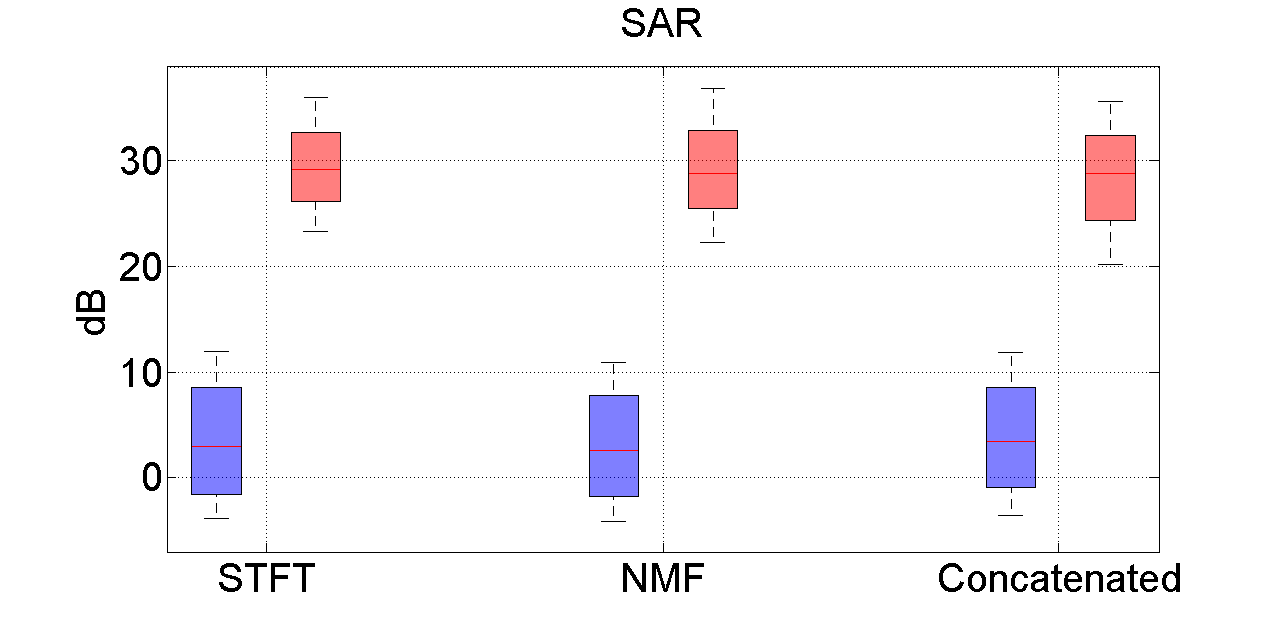
\includegraphics[width=8cm]{fig/DictSAR}
%  \caption{\label{resultsDictSAR} SAR of harmonic (left bar)/percussive (right bar) estimated sources on the SiSec database with a STFT dictionary, a NMF dictionary and their concatenation.}
%\end{figure}
%
%\begin{figure}[H]
%  \centering 
%  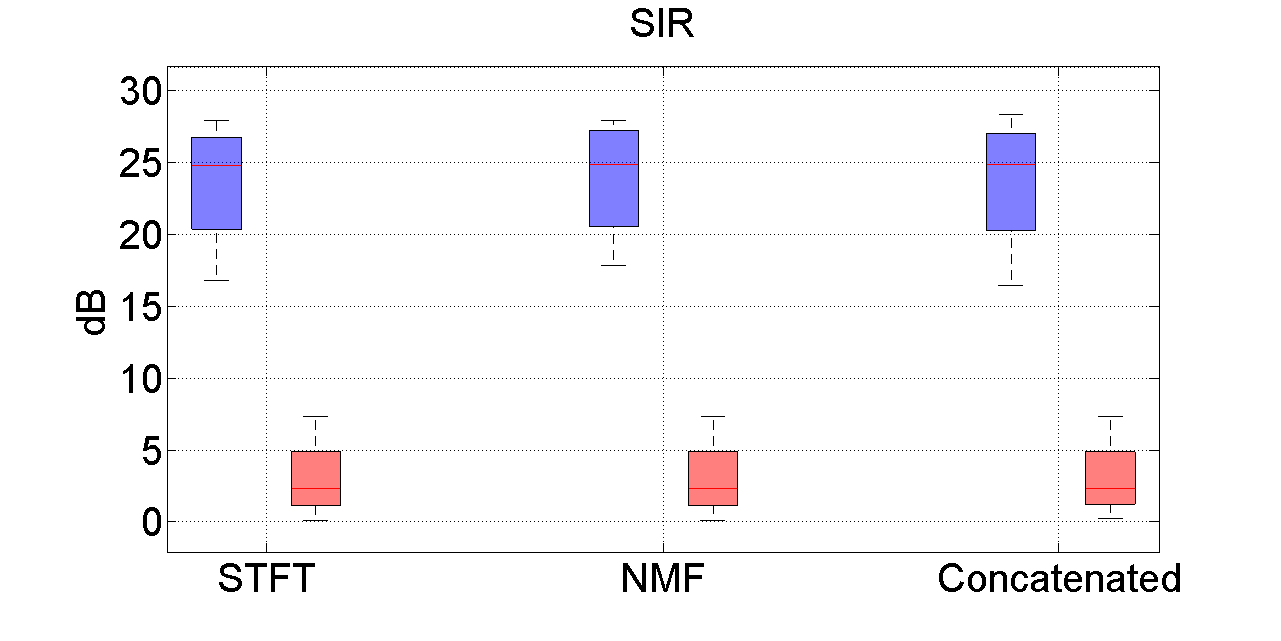
\includegraphics[width=8cm]{fig/DictSIR}
%  \caption{\label{resultsDictSIR} SIR of harmonic (left bar)/percussive (right bar) estimated sources on the SiSec database with a STFT dictionary, a NMF dictionary and their concatenation.}
%\end{figure}

\subsection{Results on the sub database}
\label{appendix:sub_database}

\begin{figure}[H]
  \centering 
  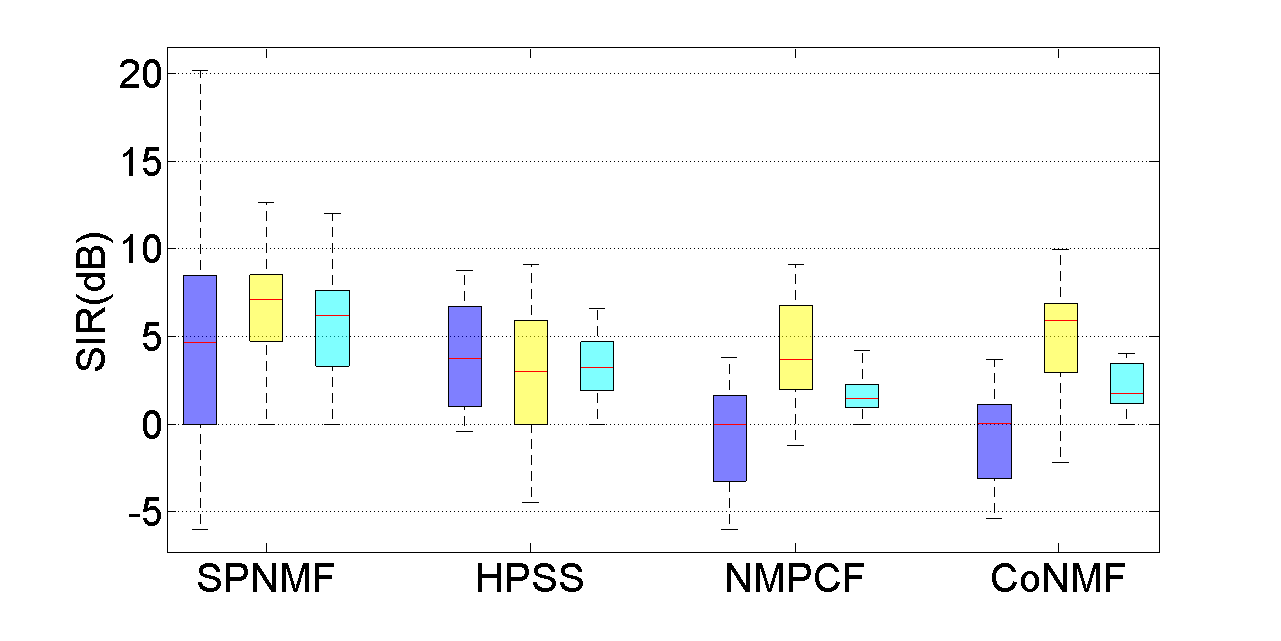
\includegraphics[width=9cm]{fig/ElectroFusionSIR}
  \caption{\label{ElectroFusionSIR} SIR for percussive/left, harmonic/middle, mean/right separation results on the Electronic/Fusion songs for the four methods.} 
\end{figure}

\begin{figure}[H]
  \centering 
  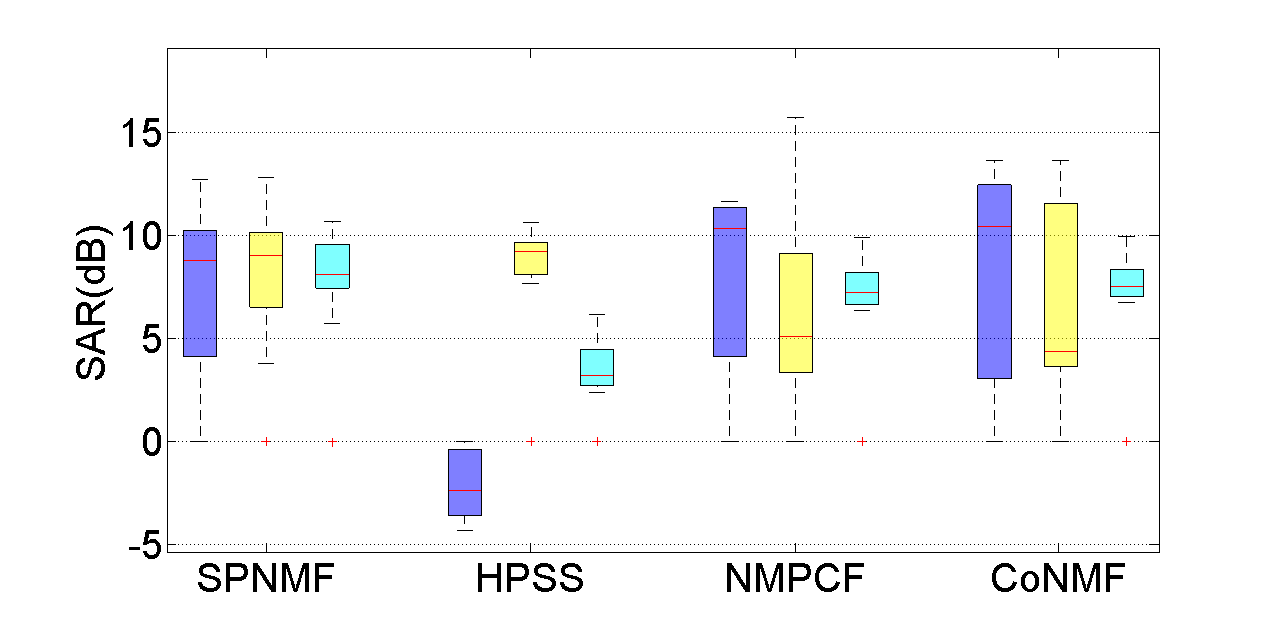
\includegraphics[width=9cm]{fig/ElectroFusionSAR}
  \caption{\label{ElectroFusionSAR} SAR for percussive/left, harmonic/middle, mean/right separation results on the Electronic/Fusion songs for the four methods.}
\end{figure}
